\chapter{引言}
\label{cha:intro}

\section{研究背景及意义}
进入 21 世纪以来,计算机技术的飞速发展为人类社会的日常生活、工业生产等方方面面带来了巨大的变化。在互联网时代的大背景下,云计算应运而生提供了一种新的 IT 服务使用、扩展和交付模式。从 2006 年 3 月亚马逊推出弹性云计算(Elastic Cloud Computing)服务至今,IaaS 作为基础的云计算资源提供形式从一个新的发展趋势已经成为当下主流。诸多传统计算业务和新兴互联网业务都已开始向云平台迁移 \cite{Armbrust:2010:VCC:1721654.1721672}。

当今 IaaS 云平台中广泛使用虚拟机作为提供计算资源的基本形式。一个运行的虚拟机被称为 ``实例'',支持按需付费计价模式的虚拟机实例称为 ``按需云实例''。业内领先的各大 IaaS 云平台,如:Amazon 的 EC2 平台 \cite{AWS}、Windows 的 Azure 平台 \cite{Azure}、Google 的 GCE 平台 \cite{GCE},都使用按需云实例的形式向云租户出租计算资源。对于云租户来说,使用按需云实例相比搭建固定的本地物理集群可以消除维护底层基础设施的人力物力开销、动态申请和释放计算资源而无需为尖峰计算需求购买大量计算设备,从而大幅减少计算成本。对于大量使用云计算资源的互联网服务提供商,如:Foursquare、Pinterest、Netflix等,愿意选择在 Amazon EC2 云平台部署服务就是因为其成本低廉、弹性扩展、易于维护的特性。尤其是对于自身动态变化的负载需求,使用按需云实例可以极大地利用按需付费的特性减少计算成本。除了大型互联网服务提供商,中小型公司、科研机构等也都乐于并且习惯于使用云平台快速部署和调整应用测试环境或是实验环境。另外,对于个人云租户来说计算成本的缩减也是非常有吸引力的。

当下,计算资源已经成为像水和电一样的基础资源。云平台作为互联网时代的基础设施通过所有云租户的共享达成了规模经济效应。搭建和维护底层计算基础架构设施的费用投入相对固定,IaaS 云平台提供商通过聚合大量云租户的计算需求可以提高其底层基础计算设备的利用率从而提升效益。通过统计复用(Statistical Multiplexing),来自不同租户的计算资源请求的波峰和波谷可以潜在地得以平滑,形成相对平稳的计算资源使用请求。然而,单纯的统计复用所能做到的计算资源使用率提升是有限的。没有调整云租户需求的方式,汇总后的计算资源请求仍然存在波峰且需求大量的计算资源。例如:当今流行的网上购物节来临之时,所有的网上零售商可能都需要请求更多的计算资源以应对大量的顾客访问请求。根据 Guy Rosen 在2010年对 Amazon EC2 云平台进行的估测 \cite{ec2dailyusage},云平台中租户对计算实例的请求是剧烈波动的。图 \ref{figure:daily_ec2_launch_counts} 给出的是估计的 2007 年至 2010 年这段时间中每天的虚拟机实例启动数量。在 2010 年 2 月和 2010 年 10 月有两次明显的尖峰计算资源请求出现。由于云平台提供商必须维护足够的硬件设施和资源以应对计算资源的峰值需求,大量的服务器节点在非峰值时段都未能被使用处于空闲状态。
\begin{figure}
  \centering
  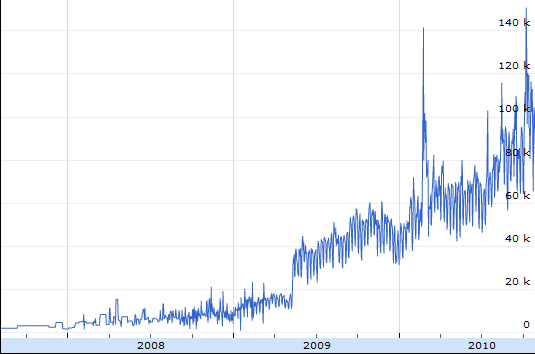
\includegraphics[width=0.9\textwidth]{cloudkick_daily_ec2_launch_counts.png}
  \caption{估测的 Amazon EC2 云平台 us-east-1 区域在 2007 至 2010 年每天的虚拟机实例启动数量 \cite{ec2dailyusage}}
  \label{figure:daily_ec2_launch_counts}
\end{figure}

没有激励云租户调整计算需求的手段,所有的计算需求可能会在同一时间堆积。如果云租户的计算需求可以被调整,将会有更大的潜力去平滑云平台中的计算资源请求。这最终可以形成对计算设备的更有效使用,提升云平台的资源使用率。虽然类似 Web 应用这类需要随时处理用户请求的实时应用很难接受这种调整,批处理任务等其它类型的应用在自身特点上是更加灵活、有弹性的。一个批处理任务通常没有时间限制或只需在一个截止期限前计算出结果就可以。这类任务可以很灵活的在计算资源可用的时候完成计算。

市场化地根据供需关系进行价格调节是非常有望促进需求转移的有效机制,云平台提供商可以通过价格信号表达云平台中当前的计算资源利用率。一个更高的价格会使可以延迟使用计算资源的云租户放弃他们当前的计算资源请求。相反地,一个更低的价格通过经济上的激励可以吸引更多的使用者。为了近一步提升计算资源利用率,IaaS 云平台提供商的旗舰 Amazon EC2 云平台已经引入了一个新的计算资源提供形式————竞价云实例。

与按需云实例不同,竞价云实例的价格根据云平台计算资源的供需关系不断变化。竞价云实例通常以极低的价格出售,但面临着随时被云平台回收的风险。当使用一个竞价云实例的时候,云租户必须首先设定一个竞价价格,作为每小时愿意支付的最大价格。竞价云实例的使用费率按每个小时开始时的竞价云实例市场价格确定。随着竞价云实例市场价格的连续波动,在该价格上升超过云租户设定的竞价价格时,云租户的竞价云实例将被关闭。直到竞价云实例市场价格升高至超过云租户设定的竞价(竞价不足失效)或者云租户主动选择关闭该节点时,该竞价云实例将结束运行。如果竞价云实例被 Amazon EC2 云平台关闭,最后不足一小时的部分将不会对云租户收取费用。如果云租户主动关闭了竞价云实例,则同使用按需云实例相同,需要支付最后不足一小时部分的费用。除了价格和可用性,竞价云实例同按需云实例是相同的。

同按需云实例一样,竞价云实例向云租户提供了足够大的实例配置类型 \cite{AWS_IT:2014} 选择空间,包括:CPU、内存、存储及网络带宽等资源的各种不同组合的硬件配置。云租户可以根据自身的应用特点和需求选择不同的实例类型。虚拟机实例分布在全球的多个地理区域 \cite{AWS_GI:2014} 中,地理区域的数量仍在继续增长中。为了保证最大程度的容错和稳定性,每个地理区域又被分成了多个隔离的空间。每个隔离的独立空间被称为一个 ``可用区''(Availability Zone)。如图 \ref{figure:aws-gi} 所示,目前 Amazon EC2 云平台有 12 个地理区域和超过 30 个可用区。本文中的应用就构建在这些可用区中,在不同可用区上的竞价云实例在价格变化和节点失效都是相互独立的。
\begin{figure}
  \centering
  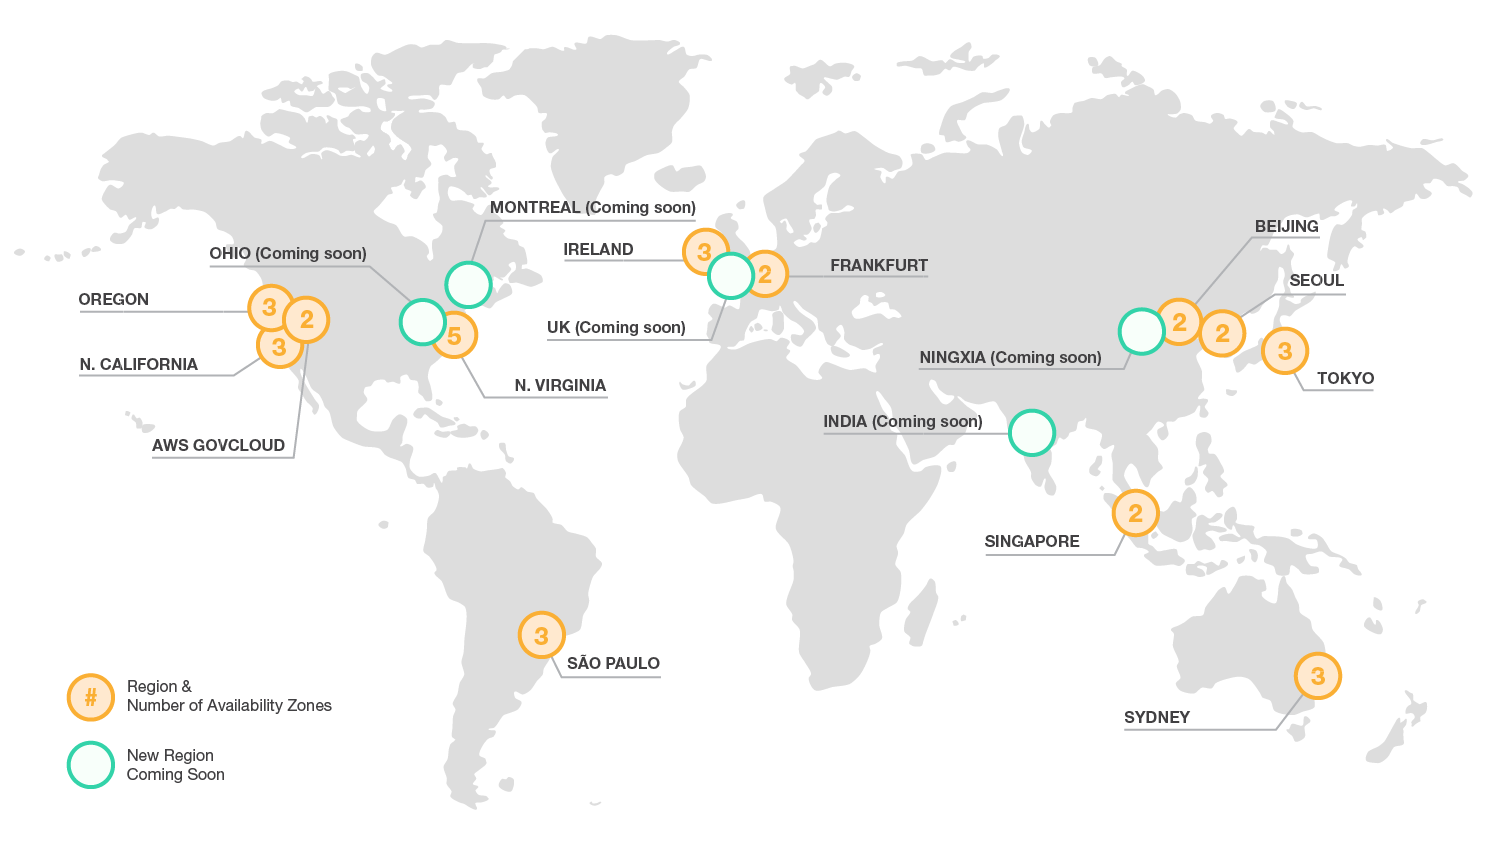
\includegraphics[width=0.9\textwidth]{Global-Infrastructure.png}
  \caption{AWS 全球基础设施地理区域和可用区概览 \cite{AWS_GI:2014}}
  \label{figure:aws-gi}
\end{figure}

要使用竞价云实例,云租户需要提交一个竞价云实例请求。在这个请求中指定实例配置类型、实例所在的可用区,以及每小时愿意支付的最大价格(被称之为 ``竞价'')。竞价云实例的市场价格由 Amazon EC2 云平台给出,价格的波动由竞价云实例资源数量的供求关系决定。图 \ref{figure:spdemo} 描述了在一段时间内竞价云实例的市场价格波动以及对某个竞价下的竞价云实例可用性的影响。当云租户给出的竞价大于等于当时的市场价格,申请的竞价云实例将启动并正常运行。显然,竞价价格设置越高竞价云实例相对越可靠、可用性越高,但又可能带来一个过高的成本。
\begin{figure}
  \centering
  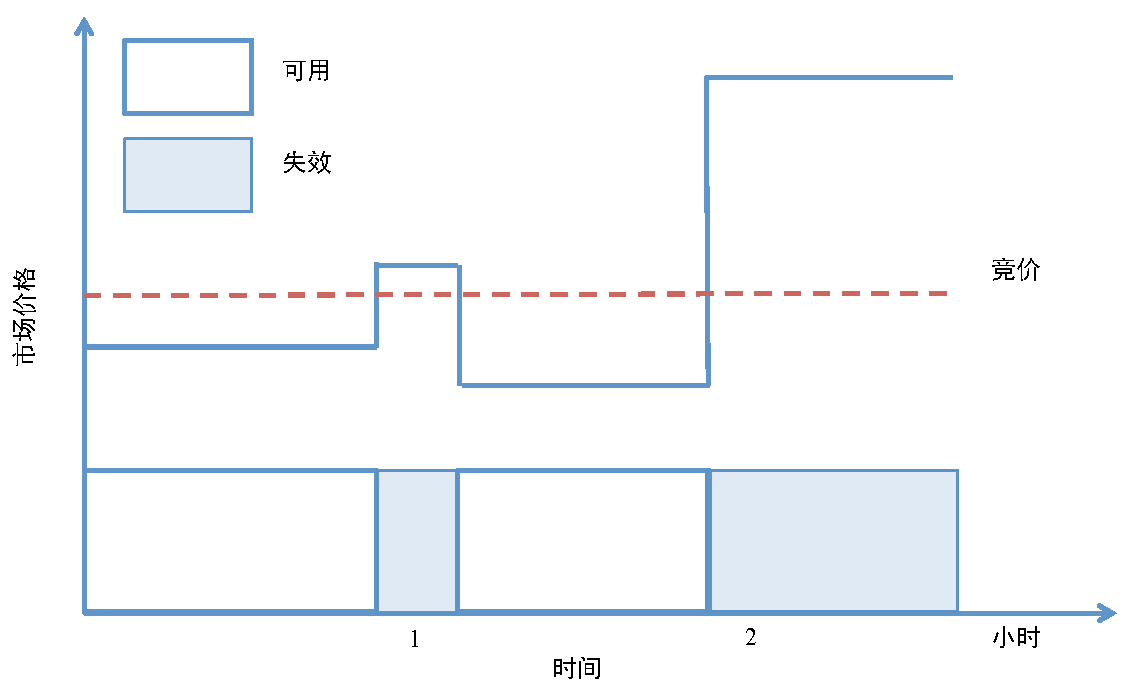
\includegraphics[width=0.85\textwidth]{spotpricedemo}
  \caption{类型竞价云实例市场价格变化示意图}
  \label{figure:spdemo}
\end{figure}

竞价云实例 \cite{SI:2014} 的出现已经给云计算带来了一个新的视野和想象空间:计算资源可以真正的如同其它商品一样在市场中根据供需关系调整价格。这对于云平台提供商来说是非常重要的一个变化:新的竞价云平台拥有了调控不同时间段计算资源使用需求的能力。对于云租户来说,通过合理设计部署在云平台中的计算应用,利用竞价云计算资源可以节省大量的计算成本。总而言之,竞价云平台的出现给云计算提供了新的活力和生机。这一变化使云平台提供商和云租户有望达成双赢的局面,并最终提高云计算资源的利用率。然而,竞价云实例本身价格波动带来的易失效特点也让云租户望而却步。直接将应用运行在竞价云实例上面临着计算的正确性、可靠性等诸多问题,而如何在不影响自身计算需求的情况下有效利用竞价云实例降低计算成本则成为了摆在所有云租户面前的一大障碍。

本文从云租户的角度出发,充分探索了竞价云平台给计算资源的使用带来的机遇和挑战。一方面利用竞价云实例有可能实现计算成本的大幅缩减,另一方面部署在竞价云实例上的应用可用性及性能得不到保障。通过对云平台中各个类型应用的分析和调研,本文认为这两方面并非是不可兼得的 ``鱼和熊掌'',而且舍弃任何一方面都将使得在竞价云平台上部署系统和应用变得毫无意义。通过对有着不同可用性要求的代表性应用有针对性地改进和设计,本文从计算机系统研究的层面给出了云租户在面对新的竞价云计算资源时如何提升在其上部署的系统的可用性及性能的方法和思路。

本研究的重要意义在于为竞价云实例的使用提供了技术基础,从而推动云租户接受、拥抱云计算的新变化。这不仅为云租户带来了大量的计算成本节约、为云平台提供商带来了计算资源使用率的提升,实现了云平台提供商与云租户的双赢。而且也间接地实现了对支撑云计算的基础设施、硬件材料、电力能源等资源的有效利用,有着深远的社会效益。

\section{面临问题与挑战}
对于云租户来说,在竞价云平台中面临的最主要问题就是如何应对竞价云实例随时可能被回收的不可靠特点。这可能导致一个正在执行的计算任务被终止造成结果数据丢失,一个正在运行的 Web 服务失效造成用户无法访问,一个分布式系统运行异常出现数据不一致。即使是利用竞价云实例作为按需云实例的补充,也可能造成系统性能的严重下降。

虽然很多系统本身有容错机制,在处理竞价云实例的节点失效上仍有不足。竞价云实例的节点失效是和市场价格以及设定的竞价相关的,这同其他的电力中断、网络拥塞、软件或硬件错误等类型故障形式极为不同,且发生频率要远高于这些常规故障。另外对于同一可用区中的两个竞价云实例来说,不论二者的竞价设定相同与否,在被回收导致的节点失效上二者是相关联的。对于需要使用大量虚拟机实例的系统来说,大量的节点关联失效也是一般容错设计上不会考虑的问题。

对于不同类型的系统来说,因各自的执行特点与需求不同,在使用竞价云实例所面临的问题与挑战也各不相同。从对竞价云实例的使用方式上,可以简单地将在竞价云平台运行的应用分为三类:1)加速任务,将竞价云实例作为性能加速器,系统中还使用可靠的按需云实例,如:大规模分布式并行处理任务;2)可中断的计算任务,如:批处理任务;3)和不可中断的、要求一直可用的服务,如:Web 服务、移动应用服务、存储服务等。具体地,又可将可中断的计算任务分为时间灵活的计算任务和有截止期限要求的计算任务两类。后者主要是那些虽没有实时性要求但超过截止期限就失去其价值的任务,如:天气预报、股票走势分析等。

对于使用竞价云实例加速大规模并行任务执行的系统,主要在于如何避免竞价云实例的加入反而拖慢了整体作业执行进度。成本和性能的权衡是在这个应用场景中主要关心的问题。如果使用竞价云实例投入的成本最终没有得到超过对应成本的按需云实例所能带来的性能提升甚至是反而带来了性能下降,那使用竞价云实例也就没有任何意义了。如:Chohan 等人 \cite{chohan2010see} 就指出:由于竞价云实例的不可靠性,直接将竞价云实例作为加速器引入一个由按需云实例组成的 MapReduce 集群可能带来负面的影响。在 MapReduce 作业执行过程中,竞价云实例节点被回收带来的相应任务重新执行会导致作业整体进度被拖慢。在这种情况下,使用竞价云实例不但无益反而有害。

运行在竞价云实例上的时间灵活、可中断的批处理任务,一般可以采用检查点等方式进行容错。但检查点或是其他容错手段一般会带来一定程度的运行时开销,以检查点为例:在批处理任务执行的某个时间点,如果不做检查点而竞价云实例被回收则会丢掉自上一个检查点到该时间点的任务进度,重新计算需要一定的计算成本;如果做检查点而竞价云实例正常运行则进行检查点的开销反而浪费了一些计算成本。如何使用、何时使用合适的容错机制是这类任务在使用竞价云实例时要解决的核心问题。有截止期限、可中断的计算任务,使用竞价云实例时需要考虑的问题则更复杂一些。一方面,虽然有截止期限但该计算任务并非要求实时处理也可以被中断,因而也可以考虑在容错和计算成本之间的权衡。另一方面,如何保证计算任务可以在截止期限之前完成也需要重点关注。

一般观点认为,不可中断的、要求一直可用的服务不应该使用竞价云实例。但实际上对于分布式服务来说,自身已经有副本状态机的容错机制可以容忍一定数量的节点错误。将这样的分布式服务部署在竞价云平台上的时候,由于节点失效模型的改变对整个分布式服务的可用性带来多大影响?可用性与计算成本之间如何权衡?这是此类本身有一定容错能力的分布式服务在竞价云平台中面临的问题。服务提供商对于成本节约的追求驱动着使用竞价云实例部署在线服务的研究,借助于竞价云平台新推出的回收告警通知特性,已经有研究者提出利用嵌套虚拟化、虚拟机活迁移等技术在竞价云实例被回收时快速切换到一个按需云实例上的方法。但如何保证在竞价云平台上在线服务仍有足够的可用性?同时是否会带来过大的性能开销?为弥补性能开销所花费的计算成本是否会超出使用竞价云实例所节约的计算成本?这些纷繁的问题对于在线服务如何利用竞价云实例提出了更加复杂且巨大的挑战。

综上,本文要解决的问题是在竞价云平台中如何根据不同类型的应用选择合适的容错机制,改进容错机制,甚至是通过对系统本身设计的修改实现在计算成本、可用性、性能三者之间的最佳平衡点。或者说在使用竞价云实例的应用节省成本的同时,如何提升各类应用的可用性和性能是本研究面临的主要挑战。

\section{研究内容与主要贡献}
\subsection{本文的研究内容}
通过对竞价云平台中相关研究现状的调研可以发现:对于可中断的计算任务如何使用竞价云实例的研究已经相对成熟,而对于包括分布式服务和在线服务在内的不可中断、要求高可用的服务如何部署在竞价云实例上的研究还十分缺乏或者是存在诸多限制。另外,MapReduce 之外的大规模计算密集型并行任务处理中如何利用竞价云实例实现性能加速也还缺少相关研究。
\begin{figure}
  \centering
  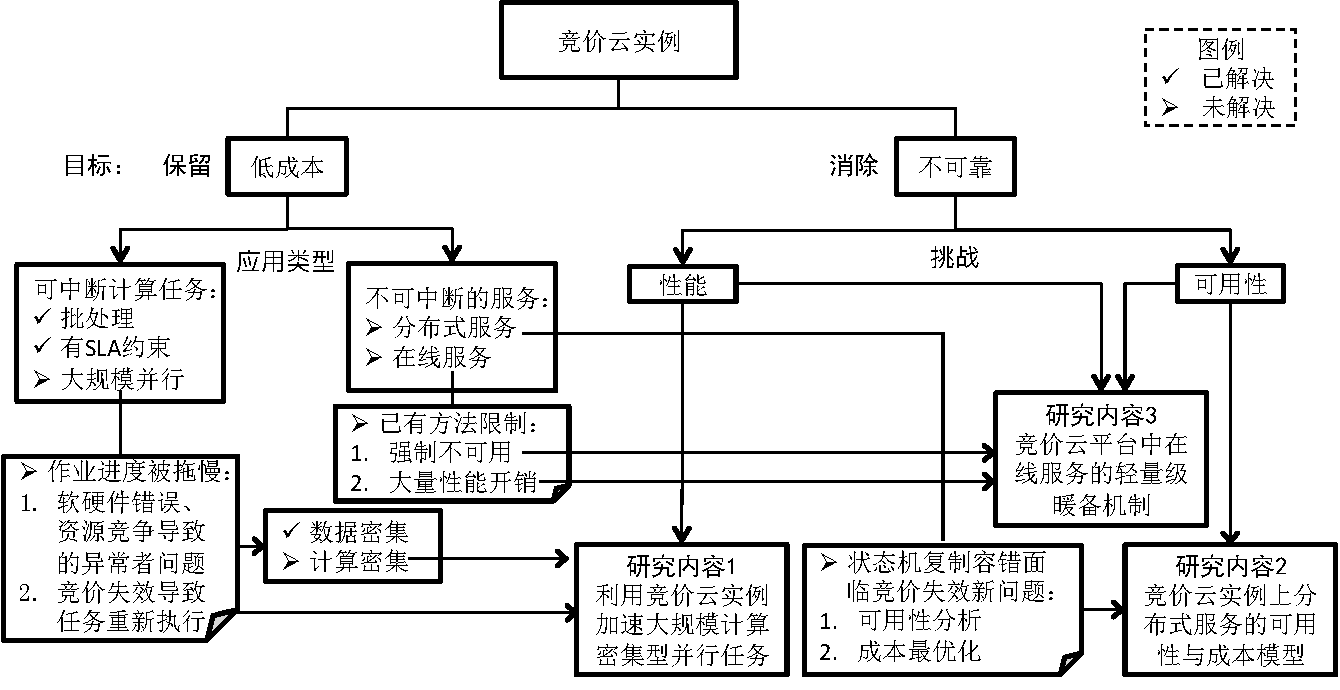
\includegraphics[width=0.9\textwidth]{proposals.pdf}
  \caption{本文研究内容概览}
  \label{figure:research_proposals}
\end{figure}

结合使用竞价云实例的各类应用所面临的不同问题和挑战,展开来说,如图 \ref{figure:research_proposals} 所示,本文的研究内容主要包括以下几个部分:
\begin{enumerate}
\item 研究如何利用竞价云平台提供的低成本计算资源加速大规模计算密集型并行任务的执行,缩减作业完成时间。这部分主要探索的是低成本的计算资源可以对大规模并行任务处理的任务调度、执行优化带来哪些变化。简单地用竞价云实例进行水平扩展可以加速作业执行,然而不可靠的竞价云实例会加剧大规模并行任务处理中的异常者拖慢整体作业进度问题。将竞价云实例用于解决异常者问题的投机执行等策略是较为恰当的使用方式,加速任务执行的同时避免了节点失效拖慢作业进度。具体地,针对一类难于预测进度的计算密集型并行任务,利用廉价的计算资源解决大规模并发时的异常者问题、加速任务执行。
\item 针对自身有容错机制的分布式服务,研究将其部署在竞价云实例上的可行性以及如何部署以达到可用性要求。由于分布式服务使用副本状态机的机制进行容错,可以容忍一部分节点失效。但竞价云实例的失效概率远高于按需云实例,使用同样多节点的分布式服务在竞价云平台中的可用性会降低很多。使用更多的竞价云实例可以提高可用性但增加了计算成本,根据此类分布式系统的可用性模型结合竞价云实例的失效特点分析分布式服务可用性与计算成本之间的关系是这部分研究的重点。
\item 基于 Amazon EC2 新推出的竞价云实例回收告警通知特性,设计在竞价云平台中提供在线服务的故障转移方法,消除现有方法的在可用性、性能上的限制。综合利用多种高可用设计和容错机制,提升竞价云平台中在线服务的可用性。减少现有方法中大量的运行时性能开销,同时在成本效率上应和现有方法的水平相当。
\end{enumerate}

\subsection{本文的主要贡献}
本文的主要贡献在于分析了竞价云平台中各类应用在计算成本、可用性、性能的潜在优化空间,探索了在使用竞价云实例的各类应用中如何提升可用性及性能,具体贡献和创新点可简要概括如下:
\begin{enumerate}
\item 针对大规模计算密集型并行计算任务中普遍存在的异常者问题,提出了基于程序跟踪和聚类分析的异常节点检测方法和基于任务克隆、投机执行、任务再分割等策略的加速执行方法。竞价云实例的使用使得这些方法在计算成本上变得可行。基于上述方法并考虑竞价云实例易失效的特点,实现了一个稳定、高效的大规模计算密集型并行任务加速器。实验评测显示该加速器在 Cap3 和 GaussianBlur 两个典型应用上可以将大规模计算密集型并行任务的作业完成时间缩减超过 20\% 和 40\%,而产生的计算成本开销只有约 3\%。
\item 指出了在竞价云平台中,分布式服务的可用性发生了较大变化。这同竞价云实例的失效特点是相关的,而竞价云实例的失效概率模型本质上是由竞价云实例的市场价格和竞价决定的。进而提出了使用竞价云实例部署分布式服务所面临的竞价决策问题的非线性规划模型,并给出了可用性和成本感知的竞价框架。该竞价框架可以在保持同按需云实例同样可用性级别的前提下大幅减少计算成本,在分布式锁服务和分布式存储服务的案例中分别得到了 81.23\% 和 85.32\% 的成本节约。
\item 提出了基于暖备对的在竞价云实例上提供在线服务的方法。这个方法消除了已有工作在可用性和性能上的限制。暖备的故障转移机制通过将服务迁移中不可控的虚拟机实例申请和启动过程移出关键路径从而消除了强制性的不可用。轻量级的迁移方法和时间可控的异步磁盘镜像极大地提高了系统性能。另外,该方法在多个地理区域、多个可用区之间从价格趋势及稳定性上综合考虑竞价策略对可用性和成本的影响。评测结果显示这个方法可以在同现有方案相近的计算成本下显著提升服务可用性和性能,在线服务的不可用性降低了接近一个数量级,在 TPC-W 和 YCSB 基准测试集上获得了至多 45\% 和 100\% 的性能提升。
\end{enumerate}

\section{全文组织结构}
本文其他各章内容组织如下:在第 \ref{cha:background} 章首先从竞价云实例的市场价格模型、利用竞价云实例执行可中断的计算任务以及如何在竞价云平台中实现高可用、高可靠等方面分析了当前竞价云实例应用优化工作的研究现状,然后对本文涉及到的子领域的相关工作做了简要介绍。在第 \ref{cha:no2} 章详细介绍了利用竞价云实例加速大规模计算密集型并行任务的方法。在第 \ref{cha:jupiter} 章形式化了在竞价云平台中部署分布式服务所面临的可用性与成本的最优化问题,并给出了综合考虑成本与可用性的竞价框架设计。在第 \ref{cha:gemini} 解释了现有利用竞价云实例提供在线服务的方法在可用性和性能上存在的诸多限制,提出了一个基于暖备的在竞价云平台上提供在线服务的轻量级容错机制。最后,在第 
\ref{cha:conclusion_futruework} 章总结了本文工作并对未来工作进行了展望。
